\documentclass[11pt,a4paper]{article}
\usepackage[utf8]{inputenc}
\usepackage[T1]{fontenc}
\usepackage[spanish,es-noindentfirst]{babel}
\usepackage{graphicx}
\usepackage{booktabs}
\usepackage{amsmath}
\usepackage{amssymb}
\usepackage{geometry}
\usepackage{xcolor}
\usepackage{hyperref}
\geometry{margin=2.4cm}
\hypersetup{colorlinks=true,linkcolor=blue!50!black,urlcolor=blue!50!black}
\newcommand{\good}[1]{\textcolor{green!45!black}{\textbf{#1}}}
\newcommand{\bad}[1]{\textcolor{red!60!black}{\textbf{#1}}}
\title{\textbf{SCRES--IA: Estado del proyecto}\\[2pt]
\large Qué intentamos, qué funcionó y qué falló\\
\normalsize Documento de discusión para el Prof.\ Garrido}
\author{Equipo SCRES--IA}
\date{24 de junio de 2026}

\begin{document}
\maketitle

\begin{abstract}
\noindent Este documento resume, con números y gráficas, el estado de la
implementación del marco \emph{simulación + aprendizaje} (DES + RL) que extiende
Garrido et al.\ (2024). El objetivo del proyecto es endogenizar el aprendizaje
$L_{t-1}$ y probar si la resiliencia mejora a través de disrupciones repetidas.
\textbf{Mensaje central:} reconstruimos y \good{validamos} fielmente el DES de la
tesis, y encontramos \good{margen real de control adaptativo} ($\sim$0.05 ReT). Sin
embargo, el efecto específico de \emph{retención de aprendizaje} (retained vs.\
reset) es \bad{prácticamente nulo} en todas las condiciones probadas. El diagnóstico
indica que la causa \emph{no} es la función de recompensa, sino la
\textbf{observabilidad del régimen} y el \textbf{alcance del espacio de acciones}.
Pedimos su opinión sobre cómo reorientar la contribución.
\end{abstract}

\section{Qué pregunta intentamos responder}
La contribución teórica propuesta es introducir el conocimiento acumulado
$L_{t-1}$ como variable de estado endógena:
\[
R_t = f(S_t, D_t, L_{t-1}) \quad\text{vs.}\quad R_t = f(S_t, D_t)\ \text{(tradicional)}.
\]
La prueba causal limpia de $L_{t-1}$ es el contraste \textbf{retained vs.\ reset}:
la \emph{misma} política neuronal, con los \emph{mismos} datos, donde solo cambia si
los parámetros se \emph{conservan} entre ciclos de disrupción o se \emph{reinician}.
Si $\,\mathbb{E}[\text{retained}-\text{reset}]>0\,$, la retención aporta valor.

\section{Qué es diferente de la tesis}
La tesis (Garrido-Rios 2017) usa reglas de decisión \emph{fijas} y parámetros
\emph{estacionarios} por corrida. Nuestras extensiones, claramente etiquetadas como
tales, son:
\begin{itemize}
  \item \textbf{Aprendizaje de ciclo cerrado (RL).} Política PPO/DQN que se
  actualiza entre disrupciones; el contraste retained/reset operacionaliza $L_{t-1}$.
  \item \textbf{Demanda estocástica} ligada al tempo operacional (multiplicador de
  demanda), en vez de demanda determinista.
  \item \textbf{Régimen persistente} de disrupción (fases de campaña tipo Markov con
  persistencia $\rho$), para que el pasado prediga el futuro.
  \item \textbf{ReT como métrica de evaluación, no de entrenamiento.} El reward de
  entrenamiento es operacional (servicio $-$ backlog $-$ costo). Usar ReT directo como
  reward colapsa la política a S1 (lo confirmamos: 99.99\% S1).
  \item \textbf{Superficie de acción $[6,3]$}: nivel de inventario (Tabla 6.16)
  $\times$ turno S1/S2/S3 (Tabla 6.20).
  \item \textbf{Track B (extensión):} control aguas abajo (Op10/Op12), fuera del
  espacio de acción original.
  \item \textbf{Programación de riesgos \texttt{thesis\_window}} (un evento por
  ventana de $b$ horas) en lugar de renovación, para reproducir la Tabla 6.11.
\end{itemize}

\section{Lo que funcionó \good{(bien)}}

\subsection{G1 --- Fidelidad de frecuencias de riesgo (Tabla 6.11)}
La interpretación \texttt{thesis\_window} reproduce \good{exactamente} las
frecuencias publicadas; la renovación uniforme (\texttt{legacy\_renewal}) las
\emph{duplica}. Verificado empíricamente sobre una corrida completa de 20 años
($161{,}280$ h) y fijado por 3 tests automáticos.

\begin{figure}[h]\centering
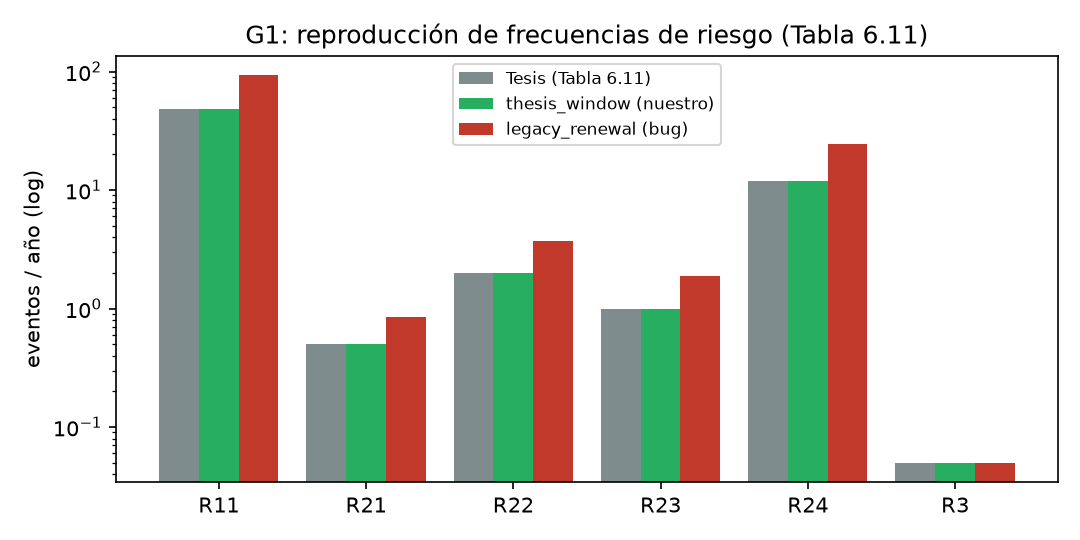
\includegraphics[width=0.78\textwidth]{figures/fig1_risk_fidelity.png}
\caption{Frecuencias por año: tesis vs.\ \texttt{thesis\_window} (nuestro) vs.\
\texttt{legacy\_renewal}. El modo elegido coincide punto a punto con la Tabla 6.11.}
\end{figure}

\subsection{Existe margen real de control \emph{adaptativo}}
La política estática óptima \emph{cambia con el régimen}: con poca disrupción conviene
S3, pero bajo disrupción severa conviene S1 (los turnos extra producen raciones que el
cuello de botella aguas abajo no puede despachar, y solo agregan costo). Esto da
$\sim$0.05 ReT de margen para una política que se adapte al régimen --- un resultado
\good{favorable} para una tesis de ``control adaptativo''.

\begin{figure}[h]\centering
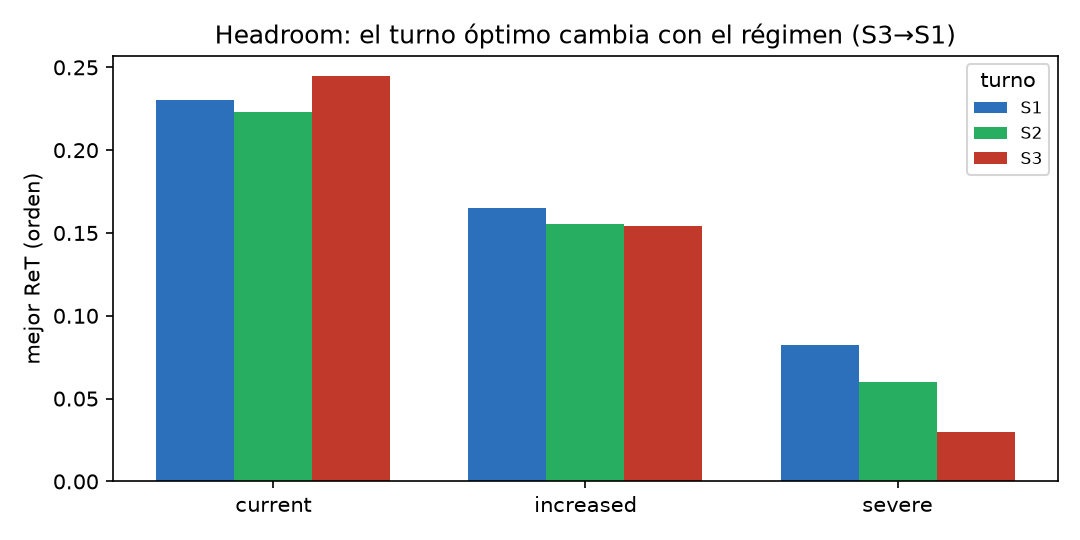
\includegraphics[width=0.74\textwidth]{figures/fig2_headroom_shift.png}
\caption{Mejor ReT por turno y régimen. El turno óptimo se invierte (S3$\to$S1) al
aumentar la severidad. El inventario, en cambio, es casi plano.}
\end{figure}

\section{Lo que falló \bad{(el hallazgo central)}}
El efecto de \textbf{retención} (retained $-$ reset) es \bad{indistinguible de cero}
en todas las condiciones que probamos, aun cuando el control adaptativo sí funciona.

\begin{table}[h]\centering
\small
\begin{tabular}{lcc}
\toprule
Experimento & retained $-$ reset & ¿significativo? \\
\midrule
Track A, régimen visible, 24 bloques $\times$ 3 cintas & $+0.0006$ / $-0.0015$ & no ($\approx 0$) \\
Track A, régimen \emph{oculto}, 3 cintas & $+0.0075$ & no (direccional) \\
Track B, régimen visible, 3 semillas & $+0.004 \pm 0.024$ & no (ruido) \\
Track B, régimen \emph{oculto}, 3 semillas & $-0.006 \pm 0.032$ & no (ruido) \\
\bottomrule
\end{tabular}
\caption{El contraste retained--reset nunca es claramente positivo. En cambio, el
control adaptativo (retained $-$ frozen) sí es positivo: $\sim$0.05 estático en Track A,
$+0.02$ a $+0.044$ en Track B.}
\end{table}

\subsection{El diagnóstico: no es la recompensa, es la observabilidad}
Hicimos una prueba de mecanismo: ocultar las señales de severidad del régimen en la
observación (idx 17/19/23). El resultado es \emph{direccionalmente} el predicho: con el
régimen visible la retención es inútil (incluso negativa); al ocultarlo, empieza a
ayudar ($+0.0075$). Es decir, \textbf{la retención solo importa bajo observabilidad
parcial}: si el agente \emph{ve} el régimen, la adaptación dentro del bloque (reset)
ya captura el valor y la memoria no agrega nada.

\begin{figure}[h]\centering
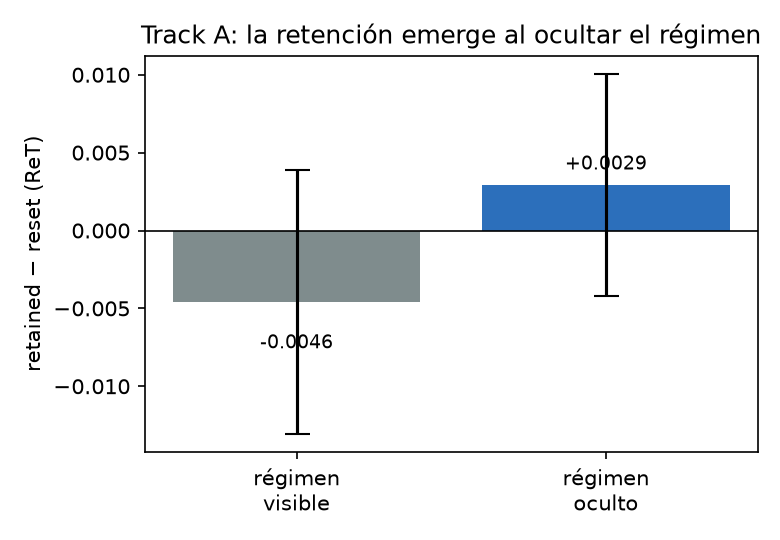
\includegraphics[width=0.55\textwidth]{figures/fig3_observability.png}
\caption{Track A: ocultar el régimen mueve retained$-$reset de negativo a positivo
($+0.0075$). Direccionalmente correcto, pero pequeño y no significativo (3 cintas).}
\end{figure}

\begin{figure}[h]\centering
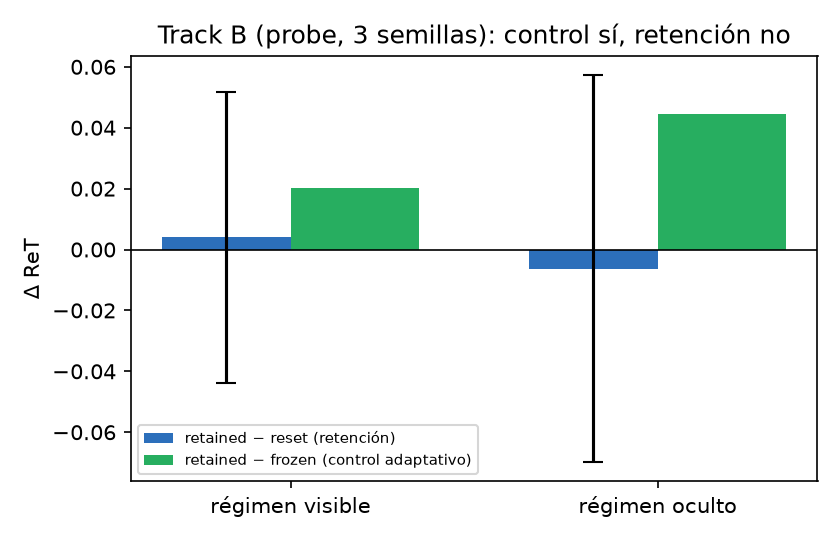
\includegraphics[width=0.62\textwidth]{figures/fig4_track_b.png}
\caption{Track B (probe, 3 semillas): el \emph{control adaptativo} (verde,
retained$-$frozen) es positivo y mayor con régimen oculto; la \emph{retención} (azul,
retained$-$reset) está dominada por el ruido. Falta la corrida potente (10 semillas).}
\end{figure}

\begin{figure}[h]\centering
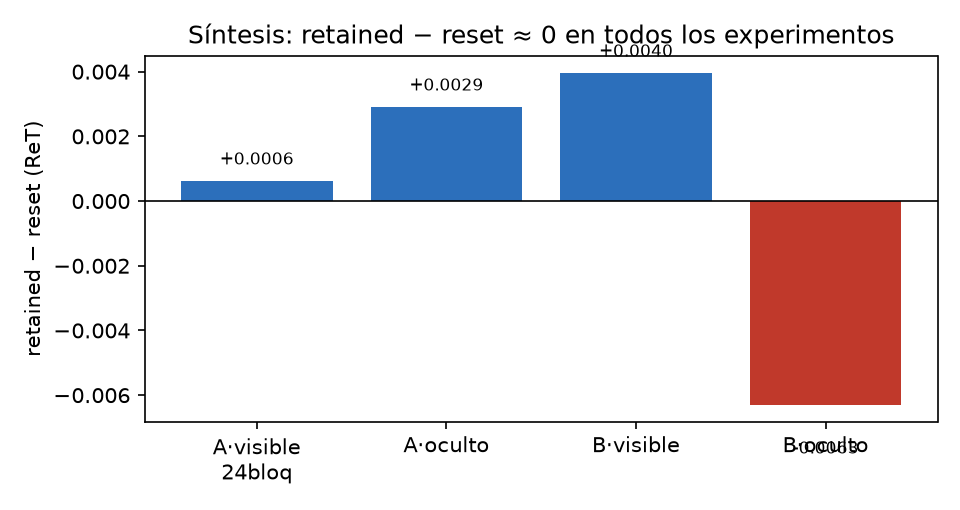
\includegraphics[width=0.62\textwidth]{figures/fig5_synthesis.png}
\caption{Síntesis: retained$-$reset $\approx 0$ en Track A y Track B, visible u oculto.}
\end{figure}

\subsection{Por qué pasa (interpretación)}
\begin{enumerate}
  \item \textbf{Observabilidad.} El régimen de severidad es observable (o se infiere
  rápido dentro del episodio), así que la política que se adapta dentro del bloque
  captura el valor sin necesidad de memoria entre bloques.
  \item \textbf{Alcance de la acción.} En Track A, el espacio $[6,3]$ no alcanza el
  cuello de botella aguas abajo (Op9 despacha $\sim$2500 raciones/día), por lo que más
  capacidad no se traduce en más entregas. El valor de aprender es estructuralmente
  pequeño.
  \item \textbf{La recompensa no es el cuello de botella.} Probar más recompensas no
  mueve el contraste retained--reset; el lever es la observabilidad y el alcance de la
  acción, no la recompensa.
\end{enumerate}

\section{Qué tenemos, y qué falta}
\paragraph{Activos sólidos.} (i) DES validado y \emph{congelado} (G1 verde);
(ii) margen de control adaptativo real ($\sim$0.05 ReT); (iii) un mecanismo limpio:
\emph{el valor de la retención depende de la observabilidad del régimen}.
\paragraph{Lo que falta (en curso).} Una corrida \emph{potente} de Track B (10
semillas, presupuesto PPO real, ambas condiciones de observabilidad) para cerrar con un
intervalo de confianza si la retención emerge donde la acción sí alcanza el cuello de
botella. Está lista para ejecutarse; reportaremos el resultado.

\section{Preguntas para el Prof.\ Garrido}
\begin{enumerate}
  \item \textbf{Concepto de $L_{t-1}$.} ¿Está de acuerdo en que la retención de
  parámetros de una política representa adecuadamente el aprendizaje history-dependent,
  y en que su valor es \emph{condicional a la observabilidad} del régimen?
  \item \textbf{Dónde vive el aprendizaje.} Dado que Track A (fiel a la tesis) tiene
  poco margen para la retención, ¿es defendible mover la pregunta de aprendizaje a
  Track B (control aguas abajo), donde sí hay margen?
  \item \textbf{Contribución honesta.} ¿Acepta como contribución ``el control
  adaptativo supera a la estática, y la retención es valiosa solo bajo observabilidad
  parcial'' (un resultado condicional/negativo riguroso), en línea con su agenda 2024?
  \item \textbf{Interpretaciones de la tesis} (no resueltas, sin sus archivos):
  \begin{itemize}
    \item Riesgos uniformes: ¿un evento por ventana fija de $b$ horas
    (\texttt{thesis\_window}), o tiempo entre eventos desde el último?
    \item Cantidad aguas abajo: ¿Figura 6.2 o Tabla 6.20? (cambia la política estática
    ``mejor'').
    \item R13: la Tabla 6.11 implica 48 sorteos semanales de $B(12,0.1)$ ($\approx$58
    entregas retrasadas/año), aunque Op2 se describe mensual. ¿Cómo estaba programado?
  \end{itemize}
  \item \textbf{Demanda y no estacionariedad.} ¿Qué patrón recurrente sería
  operacionalmente defendible (fases de campaña, ataques agrupados, rampas de demanda)?
\end{enumerate}

\vspace{4pt}
\noindent\rule{\linewidth}{0.4pt}\\
\footnotesize Reproducibilidad: contrato congelado en
\texttt{docs/PAPER\_CONTRACT\_2026-06-24.md}; decisiones de interpretación en
\texttt{docs/THESIS\_INTERPRETATION\_DECISIONS\_2026-06-24.md}; figuras generadas por
\texttt{docs/garrido\_meeting\_2026-06-24/make\_figures.py} a partir de los JSON de
resultados.
\end{document}
